
% !TEX TS-program = pdflatex
% !TEX encoding = UTF-8 Unicode

% This is a simple template for a LaTeX document using the "article" class.
% See "book", "report", "letter" for other types of document.

\documentclass[11pt]{article} % use larger type; default would be 10pt

\usepackage[utf8]{inputenc} % set input encoding (not needed with XeLaTeX)

%%% Examples of Article customizations
% These packages are optional, depending whether you want the features they provide.
% See the LaTeX Companion or other references for full information.

%%% PAGE DIMENSIONS
\usepackage{geometry} % to change the page dimensions
\geometry{a4paper} % or letterpaper (US) or a5paper or....
% \geometry{margin=2in} % for example, change the margins to 2 inches all round
% \geometry{landscape} % set up the page for landscape
%   read geometry.pdf for detailed page layout information

\usepackage{graphicx} % support the \includegraphics command and options

% \usepackage[parfill]{parskip} % Activate to begin paragraphs with an empty line rather than an indent

%%% PACKAGES
\usepackage{booktabs} % for much better looking tables
\usepackage{array} % for better arrays (eg matrices) in maths
\usepackage{paralist} % very flexible & customisable lists (eg. enumerate/itemize, etc.)
\usepackage{verbatim} % adds environment for commenting out blocks of text & for better verbatim
\usepackage{subfig} % make it possible to include more than one captioned figure/table in a single float
% These packages are all incorporated in the memoir class to one degree or another...

%%% HEADERS & FOOTERS
\usepackage{fancyhdr} % This should be set AFTER setting up the page geometry
\pagestyle{fancy} % options: empty , plain , fancy
\renewcommand{\headrulewidth}{0pt} % customise the layout...
\lhead{}\chead{}\rhead{}
\lfoot{}\cfoot{\thepage}\rfoot{}

%%% SECTION TITLE APPEARANCE
\usepackage{sectsty}
\allsectionsfont{\sffamily\mdseries\upshape} % (See the fntguide.pdf for font help)
% (This matches ConTeXt defaults)

%%% ToC (table of contents) APPEARANCE
\usepackage[nottoc,notlof,notlot]{tocbibind} % Put the bibliography in the ToC
\usepackage[titles,subfigure]{tocloft} % Alter the style of the Table of Contents
\renewcommand{\cftsecfont}{\rmfamily\mdseries\upshape}
\renewcommand{\cftsecpagefont}{\rmfamily\mdseries\upshape} % No bold!

\makeatletter
   \newcommand\figcaption{\def\@captype{figure}\caption}
   \newcommand\tabcaption{\def\@captype{table}\caption}
\makeatother
%%% END Article customizations

%%% The "real" document content comes below...

\title{CSE 523 Project Report}
\author{Arun Rathakrishnan}
%\date{} % Activate to display a given date or no date (if empty),
         % otherwise the current date is printed 

\begin{document}
\maketitle

\section{Introduction}
Given a set of points in the interval $(-1.0 ,1.0)$ given in set $S$, with center of mass at 0, the aim is to find an ordering of points $P$, such that the ordering is "good". Let $c_i$ be, the center of mass of $P$ after the $i^{th}$ point is placed. Some definitions of good are, ordering points in $P$ such that the range of $c_i$ is minimized or the total distance $c_i$ moves as each point is placed, is minimized. These are the two factors considered for evaluating any ordering in this project.\\
\\
The problem can be defined in two dimensional space if we allow the set $S$ to be defined in the domain $R \times R$. We have looked at a variant of the problem where we are allowed to pick at most $k$ points to be placed in set $P$ instead of exactly one in the original problem description. In this case, if $k$ points are picked during the $i^{th}$ attempt, we add $k$ points to $P$ and calculate center of mass $c_i$ on $P$. It has the effect of adding the center of mass of $k$ points to $P$ as a single point. Here we consider the case in which $k = 2$.

\section{Greedy Range Minimization Heuristic}
\subsection{Definition}
The heuristic aims to minimize the difference between the left most and right most values that $c_i$ can take. That is, minimize the value of $max(c_i) - \func min(c_i) $. The algorithm achieves this approximately by selecting a point such that $c_{i}$  is closest to $c_{n}$ for $i > 0$.
\subsection{Property}
	Let $c_{min}$ and $c_{max}$ represent the least and highest values of $c_i$ at any time. Then Greedy Range Minimization Heuristic ensures that no point outside the range $\left( c_{min}, c_{max} \right)$ is in selected in the set $P$ before all points within the range are selected.\\
	\\
	Consider two points $X$ and $Y$ such that both points are not selected in P till step $i-1$. Let $Y$ be outside $\left( c_{min}, c_{max} \right)$ and $X$ be inside this range. Let the center of mass values at this stage be be, $c_{i-1}$. If any point within $\left( c_{min}, c_{max} \right)$ is picked in P, it will make $c_i$ closer to $c_{n}$ than any point outside the range. Thus $X$ will always be picked ahead of $Y$ and this choice is the one that minimizes the range of center of mass and hence the property holds. \\
	\\
	Thus we can establish a relationship between reducing the interval of center of mass and the method of picking a point so that $c_i$ is closest to $c_{n}$. We can see that the heuristic takes a greedy approach to minimizing the range of $c_i$, by how it selects the next point to include in $P$.

\section{Multiple Selections}
Instead of choosing a single point, we can choose exactly 2 points at every attempt except the last one (we choose $1$ point or $2$ points).\\
\\
From a set of $n$ points let us pick $m$ sets of points $P_{k1}$, $P_{k2}$, ... , $P_{km}$. $\left\vert{P_{ki}}\right\vert = k$ , if $1 \leq i < m$, and $\left\vert{P_{km}}\right\vert \leq k$. The unordered set of points in each $P_{ki}$ are assumed to be placed at the same time. After each $P_{ki}$ is placed the center of mass changes to $c_i$.
\subsection{Property}
Let P = $P_{k1}, P_{k2}, ..., P_{km}$ be the set of points picked during $m$ attempts by heuristic $H_k$, where each set has at most $k$ points as described above. Let ${c^\prime}_1, ... , {c^\prime}_m$ be the center of masses after each attempt.  If some heuristic $H1$, which picks a single point at a time, picks point in the order $Q_1, Q_2, ... ,Q_n$, such that it is  some ordering of points in P where each point in $P_{ki-1}$ is listed before any point in $P_{ki}$, for $ki > 0$. The range of center of mass of $H_k \leq$ range of center of mass of $H_1$. $\left( {c^\prime}_{max} - {c^\prime}_{min} \right) \leq c_{max} - c_{min}.$ \\
\\
The property holds because in $H_k$ we end up selecting every $k^{th}$  $c_i$ value from $H_1$. The center of masses selected in $H_k$ is a subset of those selected in $H1$. Thus we may miss some values that are representative of the extreme points $c_{max}$ or $c_{min}$. Thus ${c^\prime}_{max} \leq c_{max}$ and  ${c^\prime}_{min} \geq c_{min}$. Hence the range of $H_k \leq$  range of $H_1$.
\section{Heuristics}
We have compared $7$ heuristics during the test runs. They appear with the heuristic number in source code.
\begin{itemize}
	\item Heuristic 0: Greedy Movement Minimization: Keep $c_i$ closest to $c_{i-1}$, picking one point a time. Greedily tries to minimize the total
	movement of $c_i$.
	\item Heuristic 1: Greedy Range Minimization: Keep $c_i$ closest to $c_n$, picking one
	point at a time.
	\item Heuristic 2: Greedy Balancing Pair (Two simultaneous selections): Pick two points at a time such that their
	average is closest to $c_n$.
	\item Heuristic 3: Greedy Range Minimization: (Two simultaneous selections): Pick two points at a time such that $c_i$ after picking two points at the $i^{th}$ attempt is closest to $c_n$.
	\item Heuristic 4: Greedy Range Minimization within $\delta$ distance: Pick two points at a time such that, if there are two points within $\delta$ distance of each other and $c_i$ after picking two points at the $i^{th}$ attempt is closest to $c_n$, the two points are picked.
	If no two points are within $\delta$ distance, pick two points without the distance restriction such that, $c_i$ after picking the two points is closest to $c_n$. The value of $\delta$ can be set upto the minimum range of $\left( c_{max}, c_{min} \right)$ found using Heuristic 1.\\
	\\
	The motivation for this heuristic is that Greedy Range Minimization may pick extreme points (both may be away from
	$c_n$), such that a heuristic which picks up points in same order but a single point at a time, may result in poor
	results for the range/ interval of center of mass. By trying to pick the early points selected in $P$, within a short
	interval, the heuristic reflects a good ordering if we evaluate the selected points as being picked one at a time.

	\item Heuristic 5: Movement Minimization with $\delta$ distance: Pick one point at a time such that, the point is within $\delta$ distance of $c_n$, and $c_i$ after picking two points at the $i^{th}$ attempt is closest to $c_{i+1}$ (Similar to Heuristic 0). If no two points are within $\delta$ distance and $c_i$ after picking a pair of remaining points is closest to $c_{i+1}$, pick those two points.
	The value of $\delta$ can be upto the minimum range of $\left( c_{max}, c_{min} \right)$ found using Heuristic 1. (In the source code, Heuristic 5 is implemented as a special case of Heuristic 0.)
	\item Heuristic 6: Movement Minimization: (Two simultaneous selections): Pick two point at a time such that, the center of mass after the $i^{th}$ attempt $c_{i-1}$ is closest to $c_i$.
\end{itemize}

\section{Results}
 For each graph show below, the experiment was run for 10 random points in the closed interval $\left( -1.0, 1.0 \right)$. In each case the range (interval) or the movement of center of mass  is compared with respect to the corresponding optimal value. The points are sorted based on their values, as a result this does not bring down the range value when we evaluate two points placed simultaneously ($c_i$ would have been decreased if we sorted points based on distance from $c_n$).
 \\
 \\
 The figure below shows the comparison of the range of center of mass with respect to the optimal value.
Greedy Range Minimization Heuristic (H1) performs better than other heuristics. The interval value from H1 is always within two times the optimal value for all test runs.
For heuristics that pick 2 points at a time, we evaluate range/interval value for Fig 1. as if the pair of points were picked one after the other.  In Fig 2. we evaluate the Movement of Center of Mass, where Greedy Movement Minimization (H0 and H5 perform equally well) outperforms other heuristics. 
\\
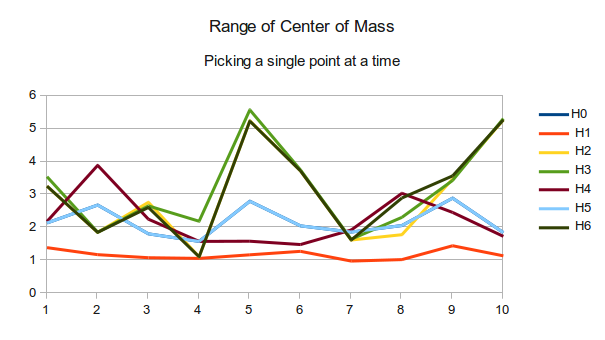
\includegraphics{result0.png}
\begin{center}
\caption{Fig 1. Range of Center of Mass}
\end{center}
\\
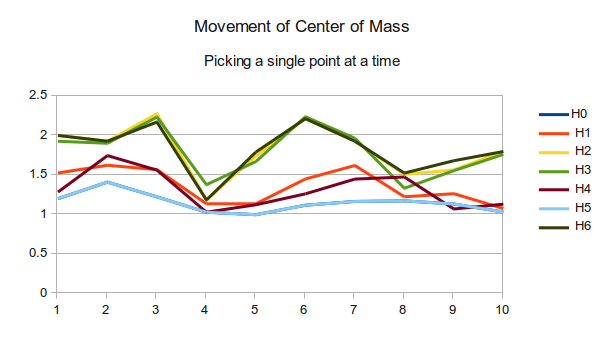
\includegraphics{result1.png}
\begin{center}
\caption{Fig 2. Movement of Center of Mass}
\end{center}
\\
\\
Fig 3. and Fig 4. show the evaluation of parameters for heuristics that simultaneously pick two points. A difference 
between picking (picking two points at a time) and ordering (consider as if pairs of points were placed one after other
in some order) is made for the sake of evaluation.
The figures compare two evaluation parameters - 2 Pick strategy and 1 Pick strategy. This shows which heuristics are better for ordering a single point at a time, though they happen to pick two points at a time.\\
\\
A motivation for considering this evaluation is that even if there is a method to place two points simultaneously on a
surface, there may be small timing errors due to which points are placed one after another in some order. The evaluation
tries to account for this.
\\
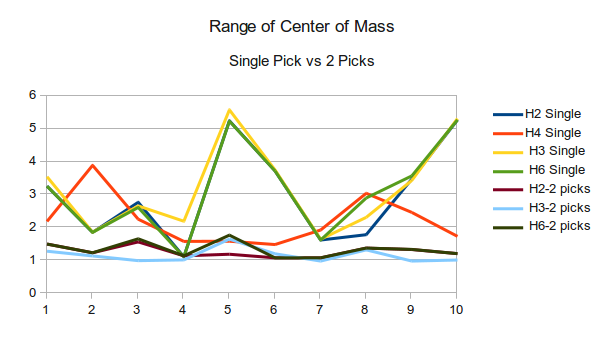
\includegraphics{result2.png}
\begin{center}
\caption{Fig 3. Range of Center of Mass}
\end{center}
Heuristic 4 (Greedy Range Minimization within $\delta$ distance) aims to keep the range of center of mass minimum but picks points within $\delta$ distance of each other first. By setting a suitable value of $\delta$ equal to the optimal values for interval ($OPT$ interval value) and distance moved ($OPT$ distance moved), we see that the single pick evaluation betters the two simultaneous points (2 pick) evaluation for Heuristic 4.\\
\\
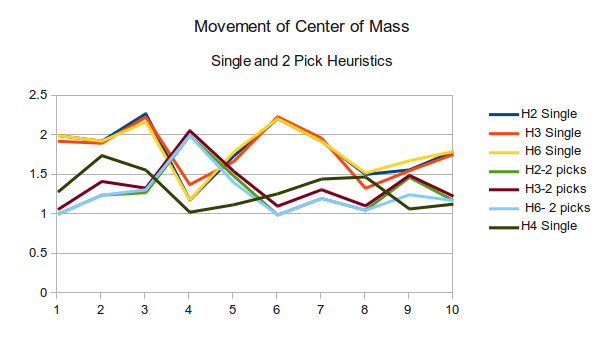
\includegraphics{result3.png}
\begin{center}
\caption{Fig 4. Movement of Center of Mass}
\end{center}
\\
\\In Fig 4. we see that H4 partitions the single pick and 2 pick evaluations for other heuristics (H2, H3 and H6). However the 2 pick evaluation for H4 (not show in the figures, but listed in results directories) has high values compared to  1 pick evaluation, though it is similar to H3 (which appears best for the interval of center of mass). H3 has the best results for 2 pick evaluation, while H4 has the worst results.

\end{document}
